% Self-contained: this file writes refs.bib on compile and inlines Figure 4.
\begin{filecontents*}[overwrite]{refs.bib}
@inproceedings{leviathan2023speculative,
  title={Fast Inference from Transformers via Speculative Decoding},
  author={Leviathan, Yaniv and Kalman, Matan and Matias, Yossi},
  booktitle={ICML},
  year={2023}
}

@inproceedings{chen2023accelerating,
  title={Accelerating Large Language Model Decoding with Speculative Sampling},
  author={Chen, Charlie and Borgeaud, Sebastian and Irving, Geoffrey and Lespiau, Jean-Baptiste and Sifre, Laurent and Jumper, John},
  booktitle={arXiv:2302.01318},
  year={2023}
}

@article{cai2024medusa,
  title={{Medusa}: Simple {LLM} Inference Acceleration Framework with Multiple Decoding Heads},
  author={Cai, Tianle and Li, Yuhong and Geng, Zhengyang and Peng, Hongwu and Lee, Jason D. and Chen, Deming and Dao, Tri},
  journal={arXiv:2401.10774},
  year={2024}
}

@article{li2024eagle,
  title={{EAGLE}: Speculative Sampling Requires Rethinking Feature Uncertainty},
  author={Li, Yuhui and Wei, Fangyun and Zhang, Chao and Zhang, Hongyang},
  journal={arXiv:2401.15077},
  year={2024}
}

@article{yang2024gateddelta,
  title={Gated Delta Networks: Improving Mamba2 with Delta Rule},
  author={Yang, Songlin and Wang, Bailin and Zhang, Yu and Shen, Yikang and Kim, Yoon},
  journal={arXiv:2412.06464},
  year={2024}
}

@article{gu2023mamba,
  title={Mamba: Linear-Time Sequence Modeling with Selective State Spaces},
  author={Gu, Albert and Dao, Tri},
  journal={arXiv:2312.00752},
  year={2023}
}

@article{qwen3,
  title={{Qwen3} Technical Report},
  author={{Qwen Team}},
  journal={arXiv:2505.09388},
  year={2025}
}

@misc{qwen38card,
  title={{Qwen3.8-27B} Model Card},
  author={{Qwen Team}},
  howpublished={Hugging Face},
  year={2026},
  note={https://huggingface.co/Qwen/Qwen3.8-27B}
}

@misc{qwen35card,
  title={{Qwen3.5-27B} Model Card},
  author={{Qwen Team}},
  howpublished={Hugging Face},
  year={2026}
}

@inproceedings{kwon2023vllm,
  title={Efficient Memory Management for Large Language Model Serving with {PagedAttention}},
  author={Kwon, Woosuk and Li, Zhuohan and Zhuang, Siyuan and Sheng, Ying and Zheng, Lianmin and Yu, Cody Hao and Gonzalez, Joseph E. and Zhang, Hao and Stoica, Ion},
  booktitle={SOSP},
  year={2023}
}

@article{zheng2024sglang,
  title={{SGLang}: Efficient Execution of Structured Language Model Programs},
  author={Zheng, Lianmin and Yin, Liangsheng and Xie, Zhiqiang and Sun, Chuyue and Huang, Jeff and Yu, Cody Hao and Cao, Shiyi and Kozyrakis, Christos and Stoica, Ion and Gonzalez, Joseph E. and Barrett, Clark and Sheng, Ying},
  journal={arXiv:2312.07104},
  year={2024}
}

@inproceedings{zhong2024distserve,
  title={{DistServe}: Disaggregating Prefill and Decoding for Goodput-optimized Large Language Model Serving},
  author={Zhong, Yinmin and Liu, Shengyu and Chen, Junda and Hu, Jianbo and Zhu, Yibo and Liu, Xuanzhe and Jin, Xin and Zhang, Hao},
  booktitle={OSDI},
  year={2024}
}

@article{lin2024qserve,
  title={{QServe}: {W4A8KV4} Quantization and System Co-design for Efficient {LLM} Serving},
  author={Lin, Yujun and Tang, Haotian and Yang, Shang and Zhang, Zhekai and Xiao, Guangxuan and Gan, Chuang and Han, Song},
  journal={arXiv:2405.04532},
  year={2024}
}

@misc{mlx2023,
  title={{MLX}: Efficient Machine Learning on {Apple} Silicon},
  author={Hannun, Awni and others},
  howpublished={https://github.com/ml-explore/mlx},
  year={2023}
}

@misc{mlxlm,
  title={{mlx-lm}},
  author={{MLX Contributors}},
  howpublished={https://github.com/ml-explore/mlx-lm},
  year={2024}
}

@misc{mlxlm990,
  title={Native {MTP} speculative decoding ({Qwen3.5}/{3.6} reference implementation)},
  author={{mlx-lm contributors}},
  howpublished={GitHub Pull Request 990},
  year={2026}
}

@misc{mlxvlm,
  title={{mlx-vlm}},
  author={Blaizzy and others},
  howpublished={https://github.com/Blaizzy/mlx-vlm},
  year={2024}
}

@misc{mlxvlm1423,
  title={Chunked {Gated DeltaNet} prefill},
  author={{mlx-vlm contributors}},
  howpublished={GitHub Pull Request 1423},
  year={2026}
}

@misc{mlxvlm945,
  title={Per-chunk \texttt{mx.eval} and \texttt{clear\_cache} stall},
  author={{mlx-vlm contributors}},
  howpublished={GitHub Issue 945},
  year={2026}
}

@misc{omlx2874,
  title={Optimal Configuration for {Qwen3.8-27B} on {M3 Max} 128{GB}},
  author={taozhiyuai and others},
  howpublished={oMLX Issue 2874},
  year={2026}
}

@misc{omlx2781,
  title={{Qwen} {ANE} Prompt Processing on {M3 Max}},
  author={{oMLX contributors}},
  howpublished={oMLX Issue 2781},
  year={2026}
}

@misc{weschera2026,
  title={{Qwen} 3.8 27{B} on {Apple} Silicon: 53--72 tok/s with {oMLX} {ANE} + native {MTP}},
  author={Weschera},
  howpublished={https://github.com/Weschera/Qwen3.8-27B-oMLX-MTP-Mac},
  year={2026}
}

@misc{ollama019,
  title={{Ollama} is now powered by {MLX} on {Apple} Silicon in preview},
  author={{Ollama}},
  howpublished={https://ollama.com/blog/mlx},
  year={2026},
  month={March}
}

@article{frantar2023gptq,
  title={{GPTQ}: Accurate Post-Training Quantization for Generative Pre-trained Transformers},
  author={Frantar, Elias and Ashkboos, Saleh and Hoefler, Torsten and Alistarh, Dan},
  journal={ICLR},
  year={2023}
}

@article{lin2024awq,
  title={{AWQ}: Activation-aware Weight Quantization for {LLM} Compression and Acceleration},
  author={Lin, Ji and Tang, Jiaming and Tang, Haotian and Yang, Shang and Chen, Wei-Ming and Wang, Wei-Chen and Xiao, Guangxuan and Dang, Xingyu and Gan, Chuang and Han, Song},
  booktitle={MLSys},
  year={2024}
}

@article{xiao2024smoothquant,
  title={{SmoothQuant}: Accurate and Efficient Post-Training Quantization for Large Language Models},
  author={Xiao, Guangxuan and Lin, Ji and Seznec, Mickael and Wu, Hao and Demouth, Julien and Han, Song},
  booktitle={ICML},
  year={2023}
}

@article{yuan2024specprefill,
  title={{SpecPrefill}: Accelerating {LLM} Prefill with Speculative Decoding},
  author={Yuan and others},
  journal={arXiv},
  year={2025}
}

@article{swiftkv,
  title={{SwiftKV}: Fast Prefill-Optimized Inference with Knowledge-Preserving Layer Skipping},
  author={Agarwal and others},
  journal={arXiv},
  year={2025}
}

@article{pyramidkv,
  title={{PyramidKV}: Dynamic {KV} Cache Compression based on Pyramidal Information Funneling},
  author={Cai and others},
  journal={arXiv:2406.02069},
  year={2024}
}

@inproceedings{dao2022flashattention,
  title={{FlashAttention}: Fast and Memory-Efficient Exact Attention with {IO}-Awareness},
  author={Dao, Tri and Fu, Daniel Y. and Ermon, Stefano and Rudra, Atri and R{\'e}, Christopher},
  booktitle={NeurIPS},
  year={2022}
}

@article{shazeer2017moe,
  title={Outrageously Large Neural Networks: The Sparsely-Gated Mixture-of-Experts Layer},
  author={Shazeer, Noam and Mirhoseini, Azalia and Maziarz, Krzysztof and Davis, Andy and Le, Quoc and Hinton, Geoffrey and Dean, Jeff},
  journal={arXiv:1701.06538},
  year={2017}
}

@article{fedus2022switch,
  title={Switch Transformers: Scaling to Trillion Parameter Models with Simple and Efficient Sparsity},
  author={Fedus, William and Zoph, Barret and Shazeer, Noam},
  journal={JMLR},
  year={2022}
}

@article{huang2024llm,
  title={A Survey on Efficient Inference for Large Language Models},
  author={Zhou, Zixuan and others},
  journal={arXiv:2404.14294},
  year={2024}
}

@misc{llamacpp,
  title={{llama.cpp}},
  author={Gerganov, Georgi and contributors},
  howpublished={https://github.com/ggerganov/llama.cpp},
  year={2023}
}

@misc{qwen31826,
  title={Chat template injects empty think tags under \texttt{enable\_thinking=false}},
  author={{QwenLM contributors}},
  howpublished={Qwen3 Issue 1826},
  year={2026}
}

@misc{mlxengine176,
  title={Prefix cache miss from {Qwen} generation-prompt think tags},
  author={{LM Studio mlx-engine contributors}},
  howpublished={mlx-engine Issue 176},
  year={2026}
}

@misc{mlxlm1077,
  title={{GDN} cache slice leak},
  author={{mlx-lm contributors}},
  howpublished={Issue 1077},
  year={2026}
}

@misc{mlxlm1162,
  title={{KVCache} offset not restored from keys},
  author={{mlx-lm contributors}},
  howpublished={Issue 1162},
  year={2026}
}

@misc{mlx3350,
  title={Small Metal free-cache forces per-layer malloc},
  author={{MLX contributors}},
  howpublished={mlx Issue 3350},
  year={2026}
}

@misc{vllm36649,
  title={\texttt{mamba\_cache\_mode=all} for hybrid {APC}},
  author={{vLLM contributors}},
  howpublished={vLLM Issue 36649},
  year={2026}
}

@inproceedings{pope2023efficiently,
  title={Efficiently Scaling Transformer Inference},
  author={Pope, Reiner and Douglas, Sholto and Chowdhery, Aakanksha and Devlin, Jacob and Bradbury, James and Heek, Jonathan and Xiao, Kefan and Agrawal, Shivani and Dean, Jeff},
  booktitle={MLSys},
  year={2023}
}

@article{patel2024splitwise,
  title={{Splitwise}: Efficient Generative {LLM} Inference Using Phase Splitting},
  author={Patel, Pratyush and Choukse, Esha and Zhang, Chaojie and Goiri, {\'I}{\~n}igo and Warrier, Brijesh and Mahalingam, Nithish and Bianchini, Ricardo},
  booktitle={ISCA},
  year={2024}
}

@misc{appleum,
  title={Unified Memory Architecture},
  author={{Apple}},
  howpublished={Apple Silicon documentation},
  year={2020}
}

@misc{stared2026,
  title={Benching local {LLMs} on {Apple} Silicon},
  author={stared},
  howpublished={https://github.com/stared/benching-local-llms-on-apple-silicon},
  year={2026}
}

@misc{terminalbytes2026,
  title={Run {Qwen3.8} 27{B} locally: real numbers from my {Mac} {Studio}},
  author={{TerminalBytes}},
  year={2026},
  howpublished={Community bench of Ollama Q4\_K\_M Qwen3.8-27B vs.\ Qwen3.6-27B on M3 Ultra}
}

@misc{orcarouter2026,
  title={{Qwen3.8-27B} on {Apple} Silicon: {MLX} Setup, {VRAM} and Reality},
  author={{OrcaRouter}},
  year={2026},
  howpublished={https://huggingface.co/orcarouter/Qwen3.8-27B-MLX}
}

@misc{ctaylor83mtp,
  title={{Qwen3.8-27B} {MTP}: the flag was free the whole time},
  author={ctaylor83},
  howpublished={https://github.com/ctaylor83/qwen38-mtp},
  year={2026}
}

@misc{zlabdflash,
  title={{DFlash2} draft models for {Qwen3.8}},
  author={{z-lab}},
  howpublished={Hugging Face},
  year={2026}
}

@article{yarn2024,
  title={{YaRN}: Efficient Context Window Extension of Large Language Models},
  author={Peng, Bowen and Quesnelle, Jeffrey and Fan, Honglu and Shippole, Enrico},
  journal={ICLR},
  year={2024}
}

@inproceedings{vaswani2017attention,
  title={Attention Is All You Need},
  author={Vaswani, Ashish and Shazeer, Noam and Parmar, Niki and Uszkoreit, Jakob and Jones, Llion and Gomez, Aidan N. and Kaiser, {\L}ukasz and Polosukhin, Illia},
  booktitle={NeurIPS},
  year={2017}
}

@article{dao2024flashattn2,
  title={{FlashAttention-2}: Faster Attention with Better Parallelism and Work Partitioning},
  author={Dao, Tri},
  journal={ICLR},
  year={2024}
}

@misc{slotbankrepo,
  title={slotbank},
  author={Heid, Andre},
  howpublished={https://github.com/Andylol111/slotbank},
  year={2026}
}

@article{mixtral2024,
  title={Mixtral of Experts},
  author={Jiang, Albert Q. and others},
  journal={arXiv:2401.04088},
  year={2024}
}

@inproceedings{rajbhandari2022deepspeed,
  title={{DeepSpeed-MoE}: Advancing Mixture-of-Experts Inference and Training to Power Next-Generation {AI} Scale},
  author={Rajbhandari, Samyam and others},
  booktitle={ICML},
  year={2022}
}

@inproceedings{he2022fastermoe,
  title={{FasterMoE}: Modeling and Optimizing Training of Large-scale Dynamic Pre-trained Models},
  author={He, Jiaao and others},
  booktitle={PPoPP},
  year={2022}
}

@article{cai2024medusafull,
  title={{Medusa}: Simple {LLM} Inference Acceleration Framework with Multiple Decoding Heads},
  author={Cai, Tianle and others},
  journal={arXiv:2401.10774},
  year={2024}
}

@misc{gemfilter,
  title={{GemFilter}: Training-Free Token Filtering for Efficient {LLM} Prefill},
  author={Anonymous},
  year={2025}
}

@misc{pflash,
  title={{PFlash}: Dropping Prompt Tokens for Faster Prefill},
  author={Anonymous},
  year={2025}
}

@article{xiao2024infllm,
  title={{InfLLM}: Training-Free Long-Context Extrapolation for {LLMs} with an Efficient Context Memory},
  author={Xiao, Chaojun and others},
  journal={arXiv:2402.04617},
  year={2024}
}

@inproceedings{dao2022flashattention2,
  title={{FlashAttention}: Fast and Memory-Efficient Exact Attention with {IO}-Awareness},
  author={Dao, Tri and Fu, Daniel Y. and Ermon, Stefano and Rudra, Atri and R{\'e}, Christopher},
  booktitle={NeurIPS},
  year={2022}
}

@misc{mlxswift225,
  title={asyncEval prefill pipeline on {M5 Max} vs {M2 Mini}},
  author={{mlx-swift-lm contributors}},
  howpublished={GitHub Issue 225},
  year={2026}
}

@misc{mlxnode68,
  title={Chunked {GDN} slower than per-step on Metal},
  author={{mlx-node contributors}},
  howpublished={GitHub Issue 68},
  year={2026}
}

@misc{sglang12867,
  title={{GDN} radix cache at \texttt{page\_size>1}},
  author={{SGLang contributors}},
  howpublished={sgl-project/sglang\#12867},
  year={2026}
}

@misc{atomgradient,
  title={{Qwen3.5-9B} Metal prefill breakdown},
  author={atomgradient},
  howpublished={mlx-inference-bench},
  year={2026}
}

@misc{nathanmaine,
  title={{Qwen3.8-27B} {MTP} on {M5 Max} 128{GB}},
  author={NathanMaine},
  year={2026},
  howpublished={https://github.com/NathanMaine/qwen-mlx-offline}
}

@misc{olmoe,
  title={{OLMoE}: Open Mixture-of-Experts Language Models},
  author={Muennighoff, Niklas and others},
  journal={arXiv:2409.02060},
  year={2024}
}

@misc{applejetsam,
  title={Responding to Low-Memory Warnings on {iOS} and {macOS} (jetsam)},
  author={{Apple}},
  howpublished={Apple Developer Documentation},
  year={2023},
  note={https://developer.apple.com/documentation/xcode/investigating-memory-access-crashes}
}

@misc{mlxlmcache,
  title={\texttt{trim\_prompt\_cache} and \texttt{can\_trim\_prompt\_cache}},
  author={{MLX Contributors}},
  howpublished={mlx-lm \texttt{models/cache.py}},
  year={2025},
  note={https://github.com/ml-explore/mlx-lm}
}

@misc{qwen35a3b,
  title={{Qwen3.5-35B-A3B} Model Card},
  author={{Qwen Team}},
  howpublished={Hugging Face},
  year={2026}
}

@misc{applemetalws,
  title={{Metal} resource limits and recommended working-set size},
  author={{Apple}},
  howpublished={Metal Programming Guide},
  year={2024}
}
\end{filecontents*}

\documentclass[11pt]{article}

\usepackage[margin=1in]{geometry}
\usepackage{times}
\usepackage{amsmath,amssymb,amsthm}
\usepackage{booktabs}
\usepackage{graphicx}
\usepackage{xcolor}
\usepackage{tikz}
\usetikzlibrary{arrows.meta,positioning,fit,calc,shapes.geometric,patterns}
\usepackage{algorithm}
\usepackage{algpseudocode}
\usepackage{hyperref}
\usepackage{natbib}
\usepackage{enumitem}
\usepackage{caption}
\usepackage{fancyhdr}
\usepackage{microtype}
\usepackage{url}
\usepackage{array}
\usepackage{placeins}

\hypersetup{
  colorlinks=true,
  linkcolor=black,
  citecolor=black,
  urlcolor=blue,
  pdftitle={slotbank: Hybrid-Safe Local Serving of Dense and Mixture-of-Experts Language Models on Low-Memory Unified Memory Devices},
  pdfauthor={Andre Heid},
  pdfsubject={Systems manuscript on local Qwen serving on a 24 GB Apple M4 MacBook Air},
  pdfkeywords={on-device LLM serving, Apple Silicon, unified memory, Gated DeltaNet, speculative decoding, prefix caching, mixture of experts}
}

\pagestyle{fancy}
\fancyhf{}
\fancyhead[L]{\small slotbank Systems Manuscript}
\fancyhead[R]{\small Heid, 2026}
\fancyfoot[C]{\thepage}
\renewcommand{\headrulewidth}{0.4pt}

\theoremstyle{definition}
\newtheorem{definition}{Definition}

\newcommand{\slotbank}{\textsc{slotbank}}
\newcommand{\gdn}{Gated DeltaNet}

\title{\vspace{-1.2em}
\textbf{slotbank}: Hybrid-Safe Local Serving of Dense and Mixture-of-Experts\\
Language Models on Low-Memory Unified Memory Devices\\[0.4em]
\large Running Qwen3.8-27B on an Apple M4 MacBook Air}

\author{
Andre Heid\\
Yale University\\
\texttt{andre.h.costa@yale.edu}
}

\date{2 September 2026 \\[0.3em] \small Systems manuscript (single-machine study)}

\begin{document}
\maketitle
\thispagestyle{fancy}

\begin{abstract}
Quantization makes modern language models small enough to fit nominally within commodity Apple Silicon memory, but nominal fit is not the same as practical serving. On a 24\,GB system, model weights, Metal allocations, the operating-system page cache, and recurrent model state compete for the same physical DRAM~\citep{appleum}. Hybrid architectures further complicate the problem: recurrent \gdn{} state cannot be paged or trimmed like a transformer KV cache~\citep{yang2024gateddelta,qwen3}, so several common serving optimizations are either unavailable or incorrect.

\slotbank{} is a single-process MLX runtime built around these constraints. It has two serving paths that share a correctness contract but not a cache. For mixture-of-experts checkpoints whose expert banks exceed the practical Metal working set, a file-backed bank stores the stacked experts and a capacity-limited \emph{slot pack} of size $C$ is the only tensor \texttt{gather\_qmm} ever sees. For dense Qwen3.8-27B, where no useful expert subset exists, that machinery is off: the same memory-first rule reduces to fitting an affine-4 target and a 66.4M-parameter multi-token-prediction sidecar within an 18\,GiB working-set budget, then retaining stock \texttt{mlx-vlm} kernels. Speculative decoding is restricted to a rollback path that can restore hybrid state. Prefix reuse restores only exact stored prefixes.

On a 24\,GB M4 MacBook Air, dense Qwen3.8-27B reaches 5.71 tok/s under greedy decoding and 9.95--13.47 tok/s with native multi-token prediction, depending on workload. An 819-token cold prefill runs at approximately 48 tok/s; exact-prefix reuse reduces follow-up time-to-first-token from 17.0\,s to 0.88\,s. Separately, Qwen3.5-35B-A3B---a 19.02\,GiB 4-bit MoE checkpoint that does not run practically under the evaluated stock configurations---reaches 4.2 tok/s cold end-to-end and 6.1 tok/s warm with a 32-slot pack and approximately 3.8\,GiB wired. Increasing that pack to 64 slots reduces expert misses by 31\% yet lowers throughput, because the additional resident memory displaces page-cache pages and increases disk traffic.

These results show that constrained unified-memory serving is not only a model-size problem. Accelerator residency, file caching, hybrid-state correctness, and prompt reuse interact strongly enough that optimizing any one of them in isolation can make the system slower or change the model being served. The study is limited to a single 24\,GB Apple Silicon platform; its contribution is the resulting systems design and the measured behavior of that design, rather than a claim of platform-independent speedup.
\end{abstract}

\vspace{0.4em}
\noindent\textbf{Keywords:} on-device LLM serving, Apple Silicon, unified memory, Gated DeltaNet, speculative decoding, prefix caching, mixture of experts

%======================================================================
\section{Introduction}
\label{sec:intro}

Serving large language models on constrained unified-memory systems is a different optimization problem from discrete-GPU inference. The relevant limit is not whether a quantized checkpoint can be loaded, but how much of the shared memory hierarchy should remain resident, how much should remain reclaimable, and which model states can be reused without changing inference semantics~\citep{appleum,kwon2023vllm}. On the 24\,GB M4 Air evaluated here, those distinctions are large enough to reverse otherwise reasonable choices.

This paper uses two model classes as separate experimental objects. They share a runtime and a correctness contract. They do not share a cache, a capacity parameter, or a headline clock.

\begin{definition}[Slot and capacity $C$]
A \emph{slot} is one resident expert in a packed Metal tensor of width $C$. The router’s expert id is remapped to a slot id; \texttt{gather\_qmm} indexes only that pack. $C$ is fixed for a generate. It is not a batch size, not a speculative block length, and not used on dense models. The measured interior optimum on Qwen3.5-35B-A3B is $C{=}32$ (\S\ref{sec:eval-moe}).
\end{definition}

\paragraph{Sparse path (MoE).}
Qwen3.5-35B-A3B is a 19.02\,GiB 4-bit checkpoint, 16.9\,GiB of it routed experts~\citep{qwen35a3b,shazeer2017moe}. Keeping more experts resident initially improves throughput. Performance peaks at a 32-slot pack and then declines. Moving from $C{=}32$ to $C{=}64$ reduces misses per call by 31\% yet increases disk traffic and lowers sustained throughput: the extra 2.1\,GiB of wired pack is taken from the page cache that was serving the remaining misses. Expert residency and file caching cannot be optimized independently on this machine.

\paragraph{Dense path (27B).}
Qwen3.8-27B exposes a different boundary of the same rule~\citep{qwen38card}. Its approximately 15\,GiB 4-bit checkpoint already fits in the practical Metal working set, so expert slots provide no useful decomposition and are not installed. The configuration is: retain the quantized target, reserve enough memory for transients, attach Qwen’s own 66.4M-parameter MTP sidecar~\citep{qwen3,mlxlm990}, and leave execution on stock \texttt{mlx-vlm}. On this Air that path reaches 5.71 tok/s greedy and 9.95--13.47 tok/s with native MTP. Those values sit close to a $120/400$ bandwidth scaling of published M3 Max Metal numbers~\citep{omlx2874}, which is evidence that the remaining decode limit is the memory system, not a missing local wrapper.

\paragraph{Hybrid correctness.}
The harder constraint is state. Qwen3.8-27B is 48 \gdn{} layers and 16 full-attention layers~\citep{yang2024gateddelta,qwen3}. Attention layers hold ordinary per-token KV. Recurrent layers hold an accumulated prefix $S_t$ with no Metal right-inverse that recovers $S_{t-k}$. In \texttt{mlx-lm}, rejected speculative drafts are supposed to disappear through \texttt{trim\_prompt\_cache}: that call is the library’s embodiment of ``rewind the cache by $n$ tokens after a rejected draft''~\citep{mlxlmcache,leviathan2023speculative}. On a hybrid \texttt{ArraysCache} the function is specified to return 0 and leave $S_t$ untouched. Generation then continues from tokens the user never saw~\citep{slotbankrepo}. Prefix reuse has the same restriction. A longest-common-prefix (LCP) cache, as in SGLang’s radix tree~\citep{zheng2024sglang}, shortens a stored transformer KV to the shared prefix of the next request. That shortening is exactly a trim. Hybrid state cannot take it. Only an \emph{exact} previously materialized prefix can be restored.

\paragraph{Exact-prefix reuse, and where the clocks come from.}
Exact-prefix reuse means: the stored token ids $p$ equal the leading ids of the new request, and the stored recurrent-plus-KV snapshot is the state after prefill of $p$. The runtime then prefills only the suffix. It does not manufacture $p$ by trimming a longer snapshot. On this Air an 819-token cold tile is 17.0\,s (${\approx}48$ tok/s). The same follow-up is 0.88\,s when that equality holds ($19{\times}$). Those two marks are not a $19{\times}$ faster QMM. The 17.0\,s figure is a cold prefill of an 819-token body, including quantized matmul and fused Metal GDN on 10 cores; variance there is thermal state and whether the 15\,GiB pack is already pinned. The 0.88\,s figure is a cache hit: the expensive prefix is skipped. It will regress to the 17.0\,s class if the next request edits history, reorders excerpts, or differs in the generation-prompt tokens Qwen injects around thinking tags~\citep{qwen31826}. Memory-reuse bugs produce the same symptom: a restored \texttt{KVCache} whose \texttt{offset} was not rewritten looks empty, the suffix is appended as a full prefill, and the clock looks like a miss even though the bytes were resident~\citep{mlxlm1162}.

\paragraph{What this runtime is, relative to Ollama and MLX.}
\slotbank{} is not a faster QMM and it is not a claim that this Air beats Ollama on a Max. Ollama is a product wrapper over llama.cpp or an MLX preview; on an M3 Ultra, Qwen3.8-27B Q4\_K\_M measures 14.0 tok/s against 28.6 for Qwen3.6-27B because hybrid kernels were immature~\citep{terminalbytes2026,ollama019}. An M4 mini without MTP measures 5--6 tok/s~\citep{orcarouter2026}, which matches this Air’s greedy 5.71. The novelty is not a higher 27B bar. It is (i)~a slot capacity $C$ that is co-designed with the OS page cache, which is what makes a 19\,GiB 35B-A3B runnable here when stock MLX thrashes and the tested llama.cpp Q4 configurations do not run; (ii)~a hybrid-safe speculate/prefix contract that uses \texttt{mlx-vlm}’s \texttt{rollback\_speculative\_cache} instead of \texttt{mlx-lm}’s no-op trim, so a tok/s gain is still the same 27B; (iii)~leaving compute on stock MLX kernels (\texttt{gather\_qmm}, fused Metal GDN) rather than reimplementing them. The 27B clocks are a characterization of that contract. The MoE interior-$C$ result is the general claim.

The contribution of \slotbank{} is therefore not a new quantizer, attention kernel, or scheduler. It is a serving design that makes the interactions above explicit and measures where the usual abstractions---larger resident caches, trimmable model state, interchangeable speculative paths---stop holding on a 24\,GB hybrid-model workload.

%======================================================================
\section{Memory and State Constraints}
\label{sec:bg}

\subsection{Unified memory is a shared hierarchy}
\label{sec:tiers}

On a discrete GPU, model residency and the host page cache are separated by distinct pools. Apple Silicon exposes the same DRAM to the CPU, GPU, and file cache~\citep{appleum,applemetalws}. Table~\ref{tab:tiers} records how that pool behaved on \emph{this} fanless 24\,GB M4 Air during the runs below. It is not a claim that every M4 Air, or every Activity Monitor snapshot, shows the same GiB split.

\begin{table}[t]
\centering
\caption{Serving tiers on the evaluated 24\,GB M4 Air. Advertised Metal working set and page-cache headroom are machine- and load-specific. Activity Monitor is a process snapshot (WindowServer, browser, and other apps included) and is not the admission oracle.}
\label{tab:tiers}
\small
\begin{tabular}{@{}lll@{}}
\toprule
Tier & This Air & Role \\
\midrule
1 Wired Metal & ${\approx}17.8$\,GiB advertised WS & Resident pack or 4-bit 27B; jetsam above the practical limit \\
2 Page cache & ${\approx}12$--16\,GiB usable & File-backed expert weights and mmap hits \\
3 SSD & remainder & Misses through \texttt{pread} / readahead \\
\bottomrule
\end{tabular}
\end{table}

The split is not an arbitrary reservation. Metal allocations are \emph{wired} because a GPU shader cannot take a page fault the way a CPU load can; the OS therefore advertises a Metal working-set cap and will jetsam a process that pushes past it~\citep{applejetsam,applemetalws}. File-backed experts can be sparse because the slot pack is the only tensor the gather kernel touches. Misses are host reads into that pack, not a second copy of the bank in wired memory. macOS also drives the free-page count toward zero by design, so ``Memory Available'' in Activity Monitor is the wrong input to admission. This runtime uses reclaimable pages (free, speculative, inactive, purgeable). Shedding a useful prefix snapshot because the free-page counter is low converts a hit into a guaranteed miss.

Decode throughput is bounded approximately by delivered bandwidth over bytes touched per token,
\begin{equation}
\tau \approx B / W_{\mathrm{touch}}.
\label{eq:tau}
\end{equation}
A 15\,GiB 4-bit pack on 120\,GB/s gives a full-pack-read ceiling of roughly $8$ tok/s. Speculative decoding can exceed that by amortizing one target forward over several accepted tokens. Moving work to the Neural Engine does not raise DRAM bandwidth and, on the published large-memory paths considered here, needs a second residency~\citep{weschera2026,omlx2874}.

Warm page-cache reads on the sparse path reach about 10\,GB/s; batched SSD readahead 1000--3300\,MiB/s; one-at-a-time mmap faults about 358\,MiB/s. The page cache is part of the serving path. Wiring more experts in order to ``use the GPU better'' can make the complete path slower.

\begin{figure}[t]
\centering
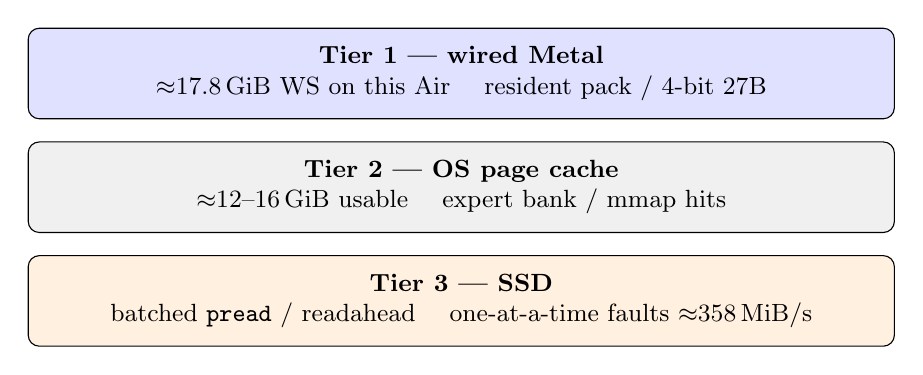
\begin{tikzpicture}[font=\small, every node/.style={align=center}]
\node[draw, rounded corners, fill=blue!12, minimum width=11cm, minimum height=1.15cm] (t1) {\textbf{Tier 1 --- wired Metal}\\${\approx}17.8$\,GiB WS on this Air \quad resident pack / 4-bit 27B};
\node[draw, rounded corners, fill=gray!12, minimum width=11cm, minimum height=1.15cm, below=0.28cm of t1] (t2) {\textbf{Tier 2 --- OS page cache}\\${\approx}12$--16\,GiB usable \quad expert bank / mmap hits};
\node[draw, rounded corners, fill=orange!12, minimum width=11cm, minimum height=1.15cm, below=0.28cm of t2] (t3) {\textbf{Tier 3 --- SSD}\\batched \texttt{pread} / readahead \quad one-at-a-time faults ${\approx}358$\,MiB/s};
\end{tikzpicture}
\caption{Three-tier view of unified memory on the evaluated Air. The MoE path limits wired slots so the rest of the bank can remain evictable pages. The dense path uses the same rule by fitting the 4-bit target and not installing slots.}
\label{fig:tiers}
\end{figure}

\subsection{Hybrid recurrent state is not a KV cache}
\label{sec:hybrid}

Qwen3.8-27B is a 64-layer hybrid with a repeating $3{:}1$ pattern: three \gdn{}+FFN blocks and one full-attention+FFN block, sixteen times (Table~\ref{tab:qwen38}, Figure~\ref{fig:hybrid})~\citep{qwen38card,yang2024gateddelta}. In the running process that is not a diagram. It is two MLX cache types in one list. Each GDN layer stores an \texttt{ArraysCache} matrix $S_t$ of $O(1)$ size (${\approx}150$\,MiB float32 for the stack). Each attention layer stores a \texttt{KVCache} at ${\approx}64$\,KiB/token. \texttt{can\_trim\_prompt\_cache} is the conjunction over that list~\citep{mlxlmcache}. One untrimmable layer makes the whole stack untrimmable, which is why paging or LRU of ``the KV cache'' is refused.

A GDN layer updates
\begin{equation}
S_t = S_{t-1}\bigl(I - \beta_t k_t k_t^\top\bigr) + \beta_t v_t k_t^\top
\label{eq:gdn}
\end{equation}
with an input-dependent decay. $S_t$ is a function of the complete prefix $x_{1:t}$. The current Metal kernel does not return the intermediates that would let a server reconstruct $S_{t-k}$~\citep{vllm36649}. Consequently a longest-common-prefix cache---store the longest state, trim back to the shared prefix of the next request---is the wrong abstraction. Only an exact stored prefix can be restored without a new recurrent kernel.

\begin{table}[t]
\centering
\caption{Qwen3.8-27B properties that constrain local serving~\citep{qwen38card,yarn2024}.}
\label{tab:qwen38}
\small
\begin{tabular}{@{}ll@{}}
\toprule
Quantity & Value \\
\midrule
Parameters & 27.78B \\
Layers / pattern & 64, $16{\times}(3{\times}\mathrm{GDN{+}FFN},\,1{\times}\mathrm{Attn{+}FFN})$ \\
Hidden / FFN & 5120 / 17408 \\
Vocab (untied) & 248320 \\
GDN heads $(QK,V)$, $d$ & $(16,48)$, 128 \\
Full-attn heads $(Q,\mathrm{KV})$, $d$ & $(24,4)$, 256 \\
Full-attn KV & ${\approx}64$\,KiB/token \\
GDN state & $O(1)$, ${\approx}150$\,MiB, float32 \\
Context (card) & 262144 native; YaRN to 1M~\citep{yarn2024} \\
Practical window on this Air & 8k--16k generate; prefix snapshot $\le 2048$ \\
MTP sidecar & trained $K{=}3$, ${\approx}66.4$M / 239\,MB \\
\bottomrule
\end{tabular}
\end{table}

\begin{figure}[t]
\centering
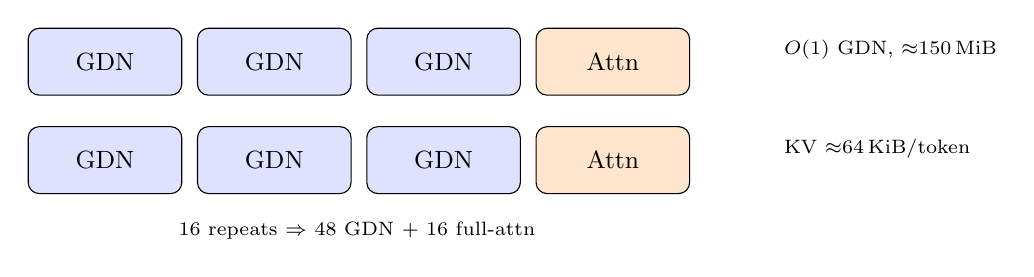
\begin{tikzpicture}[font=\small, node distance=0.18cm]
\foreach \i/\lab in {0/GDN,1/GDN,2/GDN,3/Attn} {
  \pgfmathsetmacro{\x}{\i*2.15}
  \node[draw, rounded corners, minimum width=1.95cm, minimum height=0.85cm,
        fill={\ifnum\i=3 orange!20\else blue!12\fi}] at (\x,0) {\lab};
}
\node[anchor=west, align=left, font=\scriptsize] at (8.5,0.15) {$O(1)$ GDN, ${\approx}150$\,MiB};
\foreach \i/\lab in {0/GDN,1/GDN,2/GDN,3/Attn} {
  \pgfmathsetmacro{\x}{\i*2.15}
  \node[draw, rounded corners, minimum width=1.95cm, minimum height=0.85cm,
        fill={\ifnum\i=3 orange!20\else blue!12\fi}] at (\x,-1.25) {\lab};
}
\node[anchor=west, align=left, font=\scriptsize] at (8.5,-1.1) {KV ${\approx}64$\,KiB/token};
\node[font=\scriptsize] at (3.2,-2.15) {$16$ repeats $\Rightarrow$ $48$ GDN + $16$ full-attn};
\end{tikzpicture}
\caption{Qwen3.8-27B hybrid block as implemented: sixteen repeats of three GDN layers (\texttt{ArraysCache}) and one attention layer (\texttt{KVCache}). Trim is a no-op unless every layer can rewind.}
\label{fig:hybrid}
\end{figure}

This changes speculative decode. Leviathan--Chen accepts draft token $i$ with
\begin{equation}
\alpha_i = \min\bigl(1,\, p(x_i\mid x_{<i}) / q(x_i\mid x_{<i})\bigr)
\label{eq:alpha}
\end{equation}
and must then remove rejected tokens from the target state~\citep{leviathan2023speculative,chen2023accelerating}. Trimming only the 16 KV tensors leaves rejected tokens inside the 48 GDN summaries.

\subsection{Named clocks}
\label{sec:clocks}

Four clocks appear below because they answer different questions. Mixing them is how a prefix-cache hit becomes a ``$19{\times}$ model.''

\begin{table}[t]
\centering
\caption{Clocks used in the evaluation. A number without a clock name is not comparable.}
\label{tab:clocks}
\small
\begin{tabular}{@{}p{3.6cm}p{10.2cm}@{}}
\toprule
Clock & Meaning \\
\midrule
Cold end-to-end & Tokens over wall time from process launch, including load and prefill. \\
Warm sustained decode & Tokens after the first emitted token over the measured run. \\
Time-to-first-token & Request accept to first token; here, dominated by prefill. \\
Compute-only ceiling & Sparse decode with the host-copy path stubbed; I/O vs.\ GEMM. \\
\bottomrule
\end{tabular}
\end{table}

Scaling an oMLX M3 Max Metal baseline by $120/400$ predicts 5.94 tok/s greedy and 9.78 tok/s with MTP~\citep{omlx2874}. This Air measures 5.71 and 9.95 (code). Published ANE prefill above ${+}200\%$ uses 64--128\,GB machines with a second compiled residency~\citep{weschera2026}. Those are a different memory envelope.

%======================================================================
\section{\slotbank{} Design}
\label{sec:design}

If the hot working set fits, the runtime leaves the model on stock MLX kernels. If it does not, residency is reduced before new compute kernels are introduced. An optimization that changes the target distribution is a different model, not a serving speedup. Hybrid reuse is restricted to states the runtime can restore exactly.

\begin{figure}[t]
\centering
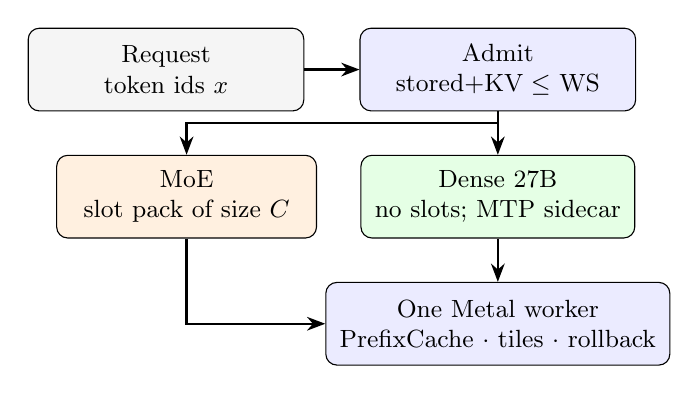
\begin{tikzpicture}[
  font=\small,
  box/.style={draw, rounded corners, align=center, inner sep=5pt, minimum height=1.05cm},
  arr/.style={-{Stealth}, thick}
]
\node[box, fill=gray!8, minimum width=3.5cm] (req) {Request\\token ids $x$};
\node[box, fill=blue!8, minimum width=3.5cm, right=0.7cm of req] (adm) {Admit\\stored${+}\mathrm{KV}\le$ WS};
\node[box, fill=green!10, minimum width=3.3cm, below=0.55cm of adm] (den) {Dense 27B\\no slots; MTP sidecar};
\node[box, fill=orange!12, minimum width=3.3cm, left=0.55cm of den] (moe) {MoE\\slot pack of size $C$};
\node[box, fill=blue!8, minimum width=4.2cm, below=0.55cm of den] (rt) {One Metal worker\\PrefixCache $\cdot$ tiles $\cdot$ rollback};
\draw[arr] (req) -- (adm);
\draw[arr] (adm) -- (den);
\draw[arr] (adm.south) -- ++(0,-0.15) -| (moe);
\draw[arr] (den) -- (rt);
\draw[arr] (moe.south) |- (rt);
\end{tikzpicture}
\caption{Request path. Dense and MoE share admission and one Metal worker. They do not share a slot pack. External chat UIs are out of scope; they are a client of the OpenAI-shaped HTTP surface, not a component of the model.}
\label{fig:arch}
\end{figure}

\subsection{Expert residency under unified memory}
\label{sec:moe-design}

A Switch-linear layer stores experts as a stack $(E,d_{\mathrm{out}},d_{\mathrm{in}})$. Stock MLX \texttt{gather\_qmm} indexes the complete stack. For Qwen3.5-35B-A3B that stack is 16.9\,GiB of a 19.02\,GiB checkpoint, so exposing it to Metal defeats the working-set limit.

\slotbank{} replaces the stack with a pack of $C$ slots (Definition~1). Installation detaches stacked tensors from each \texttt{SwitchLinear} / \texttt{QuantizedSwitchLinear}, remaps router ids to slot ids, and fills only missing experts. Dense modules are unchanged: \texttt{install\_expert\_slots} returns zero. $C$ is constant for a generate.

The pack is not sized to maximize hit rate. On 35B-A3B, $C{=}32$ wires 3.46\,GiB and $C{=}64$ wires 5.57\,GiB. The larger pack misses 31\% less often; the extra 2.1\,GiB comes out of the file cache, so remaining misses go to SSD more often and disk traffic rises. Routing is concentrated: the top 32 experts carry 53.7\% of traffic, the top 64 carry 76.2\%. The second 32 slots buy 22 points of hit rate and lose linear cache.

A slot forward is legal only when every routed expert of that forward can be resident at once. Single-token decode satisfies this. A short speculative verify is eligible only when the distinct routed set is $\le C$. Larger prefills use a path that cannot evict an expert while the same gather still depends on it. That bound is correctness, not an adaptive heuristic.

The mechanism turns off when it is unnecessary. OLMoE-1B-7B 4-bit is about 3.6\,GB and runs at 53--56 tok/s under stock \texttt{mlx-lm}~\citep{olmoe}. A 16-slot configuration cuts active memory to 1.13\,GiB and throughput to 14--19 tok/s. Slots are a fit mechanism for banks that exceed the working set, not a universal MoE accelerator.

The miss path reads into the pack layout with \texttt{os.preadv} and \texttt{memoryview}. Batched reads keep queue depth without per-page \texttt{MADV\_WILLNEED} bookkeeping. On the measured warm path, direct reads raise mean throughput from 5.820 to 7.376 tok/s across seven paired runs. The independent mmap path produces the same 100/100 token ids. A second stall was \texttt{meta[0].item()} after \texttt{mx.eval}: 224.7\,$\mu$s versus 0.8\,$\mu$s through \texttt{memoryview}. Replacing that idiom saves about 10.9\,ms/token and 6.9\% throughput without changing output.

\subsection{Dense models take a different path}
\label{sec:dense}

Dense Qwen3.8-27B has no expert subset. Applying slots or layer-streaming to a model that already fits at 4-bit adds I/O without shrinking the bytes that matter.

The default checkpoint is an affine-4 pack of about 15\,GiB (group 64). Bits per weight (bpw) is the average stored bits after quantization: 4.0 for that pack. A mixed 3.5\,bpw pack lowers peak residency to roughly 12--14\,GiB but measures only 0.94--1.11 tok/s here, because the low-bit kernels---not the wrapper---become the bottleneck. Uniform 3-bit also drops reported MMLU-Pro from 61.0 to 54.2. The dense door keeps 4-bit.

With the default 8\,GiB leave-free reserve, a 24\,GB machine exposes a 16\,GiB working set, which is not enough for 15\,GiB plus sidecar and transients. The evaluated configuration uses \texttt{--leave-free 6g} (18\,GiB). Admission checks $\mathrm{stored}+\mathrm{KV}\le \mathrm{total}-\mathrm{leave\text{-}free}$ before load. The vision tower adds about 0.4\,GiB when enabled. During large prefills the MLX free-cache is raised from 512\,MiB to 2\,GiB to avoid repeated Metal allocation, then restored~\citep{mlx3350}.

Loading and readiness are separated. The engine mmaps and builds graphs before it reports the model, then pins the 15\,GiB pack (${\approx}30$\,s). The first generate still waits if it arrives early. Restarting the process pays the pin again. That cost is reported separately from warm decode.

\subsection{Hybrid-safe speculative decoding}
\label{sec:spec}

\texttt{mlx-lm}’s \texttt{speculative\_generate\_step} rewinds rejects with \texttt{trim\_prompt\_cache}. On hybrid \texttt{ArraysCache} that rewind does not happen and the caller is not told~\citep{mlxlmcache,slotbankrepo}.

\begin{algorithm}[t]
\caption{Unsafe rewind on an untrimmable hybrid cache}
\begin{algorithmic}[1]
\State \textbf{on reject:} \texttt{trim\_prompt\_cache}(target, $n_{\mathrm{draft}}-n_{\mathrm{accept}}$)
\If{not \texttt{can\_trim\_prompt\_cache}}
  \State \Return $0$ \Comment{rejected draft state remains}
\EndIf
\end{algorithmic}
\end{algorithm}

The production path uses \texttt{mlx-vlm}’s \texttt{generate\_step} and \texttt{rollback\_speculative\_cache}. Native Qwen MTP is a 66.4M sidecar trained for block size $K{=}3$: the drafter proposes $K$ extra tokens per target forward~\citep{qwen3,mlxlm990}. $K$ is a property of the sidecar, not a serving knob. DFlash2 is a valid alternative with trained $K{=}8$ and about 1\,GiB more parameters; it is slower on both matched 27B workloads. KV quantization is off whenever a draft model is active, because the verifier reads \texttt{keys.shape}.

MTP is Qwen’s own trained head, not a third-party tree. On this 27B it is the production draft because it won a same-prefix A/B against DFlash2. It does not make 27B into a 30 tok/s model on 120\,GB/s. An always-accept $K{=}3$ ceiling is about 17 tok/s. Thirty-plus tok/s on this bandwidth is Qwen3.5-4B (32.68 greedy; 46.39 / 54.32 with DFlash at that model’s trained $K{=}5$), a different reference execution (Table~\ref{tab:4b}). Attaching the 4B as a 27B drafter is refused: different width and vocabulary, and the trim path is unsafe. Running 4B \emph{instead of} 27B is a model swap, not a serving speedup. Forcing MTP past its trained $K$ (block 6 on the 4B control) reduced throughput below baseline.

Session reuse is checked after draft. If accepted tokens cross end-of-sequence, attention offsets can run past the ids recorded as fed. The session check requires every attention-layer offset to equal $|{\mathrm{fed}}|$; otherwise the cache is dropped.

Verifying a drafted block through a $T{>}1$ GDN backbone is also refused. On Qwen3.5-4B, $\max|\Delta\mathrm{logit}|=1.562{\times}10^{-1}$; on the 35B, about 4\% of argmax decisions flip. The specialized mlx-vlm GEMV verify matches byte output on the 4B control (273 bytes at draft blocks 2 and 4).

\subsection{Exact-prefix state reuse}
\label{sec:prefix}

The live cache can be appended only when previously fed ids are a proper prefix of the new encode. A longest-common-prefix server would trim a longer snapshot; this runtime will not (Algorithm~\ref{alg:prefix}).

\begin{algorithm}[t]
\caption{Exact-prefix reuse without partial trimming}
\label{alg:prefix}
\begin{algorithmic}[1]
\State $(r,\mathrm{feed})\leftarrow \mathrm{draft\_feed}(f,x,\mathrm{hasCache})$
\If{$r>0$} \Return $(r,\mathrm{feed})$
\EndIf
\If{stored prefix $p$ exists $\wedge$ $|p|\ge 32$ $\wedge$ $p=x_{1:|p|}$}
  \State restore $s_{|p|}$ into a new cache
  \State \Return $(|p|,\, x_{|p|+1:})$
\EndIf
\State \Return $(0,x)$
\end{algorithmic}
\end{algorithm}

Qwen’s chat template creates false prefix boundaries~\citep{qwen31826}. The generation-prompt flag can insert empty thinking tags that later history does not contain; a local \texttt{/no\_think} suffix appears only on the last user turn. The stored snap is taken on the pre-\texttt{/no\_think} body so the next encode can still match.

Snapshot size is bounded because recurrent and KV state are real DRAM. A 10k-token snapshot added about 790\,MiB and triggered \emph{jetsam}: the macOS kernel killed the process under memory pressure~\citep{applejetsam}. The current maximum snapshot is 2048 tokens with a default 384\,MiB cache budget. That is the practical prefix-reuse window. The model card’s 256k / 1M context~\citep{yarn2024} is not available as a resident cache on this Air. Generate-time KV at 64\,KiB/token implies roughly 8k--16k of comfortable decode before the working set fights the 15\,GiB pack; 32k is a stretch. Restoration rewrites KV \texttt{offset} from the restored key length~\citep{mlxlm1162}. Prefill is tiled with \texttt{async\_eval}, one terminal synchronization at snapshot points, and one cache clear after the sequence~\citep{mlxvlm945}. Tiles use \texttt{skip\_logits=True} so the 248k-way head is not evaluated for intermediate positions.

\paragraph{Case study, not a contribution: long client prompts.}
Coding agents sometimes send 26k--39k-token dumps. This runtime’s HTTP surface accepts them. What Metal prefills is a bounded projection (system $\le 256$ tokens, packed ids $\le 8192$) so the 27B is not asked to materialize a hosted-API prompt. Disk keeps the verbatim dump. That split is a product choice with unmeasured task quality. It is not treated as a model contribution below.

\subsection{Executable exclusions}

Several failures are easy to reintroduce because the isolated optimization looks reasonable. The strategy catalog in the repository records adopted and rejected routes. A closed check fails if a rejected id is marked adopted, if an adopted path needs cache trim or new target weights, or if daily draft is no longer sidecar MTP. The catalog is policy, not a novelty claim.

%======================================================================
\section{Implementation and Measurement}
\label{sec:impl}

\slotbank{} is one process with one MLX worker. Metal arrays stay on the thread that created them. Only the runtime, expert-slot, and offload-cache modules may import MLX. Admission, the catalog, and the context log can therefore be checked on a host that cannot pin 15\,GiB.

A configured drafter forces \texttt{mlx-vlm}, where hybrid rollback exists. Streaming output passes through a holdback filter that separates reasoning, final content, and stop tags before text is returned.

\subsection{Evaluation platform}

All uncited 27B and 35B hardware numbers use Table~\ref{tab:host}. The study is one machine. Published larger-Mac numbers are named comparisons, not a pooled baseline.

\begin{table}[t]
\centering
\caption{Evaluation platform. Unified-memory GiB, Metal working set, and 120\,GB/s are this Air. Another 24\,GB M4 Air should be close; Activity Monitor during an unrelated snapshot will not be.}
\label{tab:host}
\small
\begin{tabular}{@{}ll@{}}
\toprule
Item & Value \\
\midrule
Machine & Fanless MacBook Air, M4 \\
Unified memory & 24\,GB \\
GPU cores (approx.) & 10 \\
Memory bandwidth & 120\,GB/s \\
Page size & 16\,KiB \\
Metal advertised WS & 17.76--17.8\,GiB \\
OS admission input & reclaimable pages, not raw free \\
MoE benches & MLX 0.32.1 / mlx-lm 0.31.3 \\
Dense 27B loader & mlx-vlm (\texttt{generate\_step} + rollback) \\
\bottomrule
\end{tabular}
\end{table}

\begin{table}[t]
\centering
\caption{Checkpoints. The 4B and OLMoE rows are \emph{controls}: a smaller dense model that can exceed 30 tok/s, and an MoE whose bank already fits so slots should lose. $K$ is the trained draft length of that sidecar, not a shared constant.}
\label{tab:ckpt}
\small
\begin{tabular}{@{}llll@{}}
\toprule
Id & Size & Role & $K$ \\
\midrule
Qwen3.8-27B-4bit & ${\approx}15$\,GiB & Dense target & --- \\
Qwen3.8-27B-MTP-4bit & 239\,MB / 66.4M & Native sidecar & 3 \\
Qwen3.8-27B-DFlash2-4bit & ${\approx}1$\,GiB & Alternative student & 8 \\
Qwen3.8-27B mixed 3.5\,bpw & 12--14\,GiB peak & Quality pack & --- \\
Qwen3.5-35B-A3B-4bit & 19.02\,GiB (16.9 exp.) & Sparse working-set case & --- \\
OLMoE-1B-7B-4bit & 3.6\,GB & Negative MoE control & --- \\
Qwen3.5-4B-4bit $\pm$ DFlash & 2.7--2.9\,GiB & Dense throughput control & 5 \\
\bottomrule
\end{tabular}
\end{table}

Page-cache state is the main confounder on the sparse path. An ordered pair $(C{=}32$ then $C{=}64)$ makes $C{=}64$ look faster because the first run warmed the bank. \emph{Alternating A/B} here means: interleave the two treatments against an already-warm page cache and report every repeat, not a product A/B test with users. Dense decode ceilings turn thinking and vision off so emitted-token rates are comparable; daily serve can leave both on.

Software invariants (import fence, catalog, recorded pins) are checked by a dated host-side script (\texttt{scripts/verify\_paper.py}, campaign \texttt{20260902T001357Z}). That campaign is a drift check on a Linux host with no Metal weights. It does not regenerate Air tok/s and it is not a second hardware evaluation. Hardware clocks remain pins in \texttt{M4\_AIR\_24G}.

%======================================================================
\section{Evaluation}
\label{sec:eval}

\subsection{Dense Qwen3.8-27B}
\label{sec:eval-27b}

Table~\ref{tab:27b} uses a cool 24\,GB M4 Air and a 64-token warm window. MTP and DFlash2 share the same greedy prefix. Published rows are other loaders, not a meta-average.

Native MTP is $2.36{\times}$ greedy on a high-acceptance count prompt and $1.74{\times}$ on code. DFlash2 ($K{=}8$) carries about four times the sidecar memory and does not pay it back on either matched workload. Always-accept $K{=}3$ is near 17 tok/s. Claims of 30--70 tok/s 27B decode on 120\,GB/s require a different model, bandwidth, or residency.

\begin{table}[t]
\centering
\caption{Qwen3.8-27B on this Air and published same-class systems. Air rows are a one-prefix pilot.}
\label{tab:27b}
\scriptsize
\begin{tabular}{@{}llrll@{}}
\toprule
Pack / path & Machine & tok/s & Peak & Note \\
\midrule
3.5\,bpw stock & Air 24\,GB & 0.94--1.11 & 12.8--14.2\,GiB & kernel-limited \\
4-bit greedy & Air 24\,GB & \textbf{5.71} & 14.4\,GiB & dense baseline \\
4-bit + DFlash2 $K{=}8$ & Air 24\,GB & 11.76 / 9.10 & 16.5--17.0\,GiB & alternative draft \\
4-bit + MTP $K{=}3$ & Air 24\,GB & \textbf{13.47 / 9.95} & 14.9--15.1\,GiB & production draft \\
4-bit greedy & M4 mini & 5--6 & --- & \citet{orcarouter2026} \\
Ollama Q4\_K\_M & M3 Ultra & 14.0 & --- & 3.8 $<$ 3.6's 28.6~\citep{terminalbytes2026} \\
oMLX ANE+MTP & M4 Max 128\,GB & 53--72 & --- & \citet{weschera2026}; no 24\,GB \\
mlx-vlm MTP & M5 Max 128\,GB & 47 & 15.5\,GB & \citet{nathanmaine} \\
\bottomrule
\end{tabular}
\end{table}

\begin{table}[t]
\centering
\caption{Smaller-model throughput control on the same Air. Output is that model’s output.}
\label{tab:4b}
\small
\begin{tabular}{@{}llrl@{}}
\toprule
Pack & Path & tok/s & Peak \\
\midrule
Qwen3.5-4B-4bit & stock mlx-vlm & 32.68 & 2.69\,GiB \\
+ DFlash $K{=}5$ & \texttt{--draft} & 46.39 / 54.32 & 2.87\,GiB \\
Qwen3.5-9B-4bit + DFlash & same & 13.75 & 5.70\,GiB \\
Qwen3.8-27B-4bit + MTP & $K{=}3$ & 13.47 / 9.95 & 14.9--15.1\,GiB \\
Qwen3.8-27B-4bit + DFlash2 & $K{=}8$ & 11.76 / 9.10 & 16.5--17.0\,GiB \\
\bottomrule
\end{tabular}
\end{table}

\subsection{Prefill and exact-prefix reuse}

An 819-token body takes 17.0\,s (48.2 effective tok/s). Reusing an exact stored prefix reduces the same follow-up class to 0.88\,s (Table~\ref{tab:prefill}). First-pass affine-4 QMM did not become $19{\times}$ faster. On 10 cores, 48 tok/s is only about $8{\times}$ greedy decode; quantized matmul remains the floor once Metal GDN is fused.

\begin{table}[t]
\centering
\caption{Prefill and follow-up clocks for an 819-token prefix.}
\label{tab:prefill}
\small
\begin{tabular}{@{}lrr@{}}
\toprule
Condition & Seconds & Effective tok/s \\
\midrule
Cold 27B tile & 17.0 & 48.2 \\
Same prefix reused (exact) & 0.88 & --- ($19{\times}$) \\
Bandwidth floor ($4{\times}15$\,GiB / 120\,GB/s) & ${\approx}0.5$ & --- \\
\bottomrule
\end{tabular}
\end{table}

\subsection{Serving an MoE checkpoint beyond the practical working set}
\label{sec:eval-moe}

At matching 4-bit quality, the evaluated llama.cpp configurations fail, pressure, or Metal-OOM. Stock \texttt{mlx-lm} thrashes at about 0.005 tok/s. The tested \texttt{mlx-vlm} load is killed. With $C{=}32$, \slotbank{} reaches 4.2 tok/s cold end-to-end to 256 tokens and 6.1 tok/s warm at ${\approx}3.8$\,GiB wired (Table~\ref{tab:moe}). Cold start pays about 19\,s of load and prefill before the second token (Table~\ref{tab:wall}). This is feasibility at this quality, not a daily 30 tok/s coder. A smaller UD-IQ4\_XS llama.cpp pack would likely fit and is a different checkpoint.

\begin{table}[t]
\centering
\caption{Qwen3.5-35B-A3B 4-bit (19.02\,GiB) on this Air.}
\label{tab:moe}
\small
\begin{tabular}{@{}llll@{}}
\toprule
Runtime & Result & Active & Notes \\
\midrule
llama.cpp (5 configs) & cannot run & OOM / pressure 4 & matching Q4 \\
stock mlx-lm & 0.005 tok/s & 18.2\,GiB & thrash \\
mlx-vlm 0.6.15 & no tokens & killed in load & free memory collapsed \\
\slotbank{} $C{=}32$ & 4.2 cold / 6.1 warm & ${\approx}3.8$\,GiB wired & 256 tokens \\
\bottomrule
\end{tabular}
\end{table}

\begin{table}[t]
\centering
\caption{35B-A3B, $C{=}32$, wall from process launch.}
\label{tab:wall}
\small
\begin{tabular}{@{}rrrr@{}}
\toprule
$N$ tokens & Wall from launch & Cold e2e tok/s & Warm decode \\
\midrule
32 & 18.7\,s & 1.71 & 5.5 \\
64 & 32.8\,s & 1.96 & 4.7 \\
128 & 42.1\,s & 3.05 & 5.6 \\
256 & 61.2\,s & 4.19 & 6.07 \\
\bottomrule
\end{tabular}
\end{table}

\subsection{Resident capacity has an interior optimum}

Table~\ref{tab:csweep} is the unified-memory result. Throughput improves from $C{=}8$ through $C{=}32$ and then falls as extra wired slots displace file-cache pages. Alternating warm runs (Table~\ref{tab:c3264}) show the mechanism: $C{=}64$ takes fewer misses and more disk. If the entire bank fits in DRAM, the trade reverses and stock kernels win (OLMoE).

\begin{table}[t]
\centering
\caption{35B-A3B capacity sweep after the read-path work. Two cold/warm reps except $C{=}96$.}
\label{tab:csweep}
\small
\begin{tabular}{@{}rrll@{}}
\toprule
$C$ & Active & Cold e2e (2 reps) & Warm decode \\
\midrule
8 & 1.88\,GiB & 3.32 / 4.19 & 4.54 / 5.78 \\
16 & 2.41\,GiB & 4.06 / 4.30 & 5.62 / 6.02 \\
\textbf{32} & \textbf{3.46\,GiB} & \textbf{4.10 / 4.88} & \textbf{5.97 / 7.15} \\
48 & 4.52\,GiB & 3.55 / 4.57 & 5.20 / 6.80 \\
64 & 5.57\,GiB & 3.36 / 3.78 & 4.84 / 5.27 \\
96 & 7.68\,GiB & 3.32 & 4.82 \\
\bottomrule
\end{tabular}
\end{table}

\begin{table}[t]
\centering
\caption{Alternating $C{=}32$ vs.\ $C{=}64$ on a warm page cache, $n{=}3$.}
\label{tab:c3264}
\small
\begin{tabular}{@{}lccc@{}}
\toprule
$C$ & tok/s & Miss/call & Disk MiB/tok \\
\midrule
32 & 8.60 / 8.74 / 8.53 & 3.012 & 17.1 / 15.5 / 22.0 \\
64 & 7.35 / 6.31 / 5.93 & 2.089 & 24.2 / 39.0 / 41.5 \\
\bottomrule
\end{tabular}
\end{table}

\subsection{Why sparse I/O work matters}
\label{sec:eval-io}

The 35B result is not a new expert kernel. It is the same \texttt{gather\_qmm} on a pack that can actually be filled without thrashing. Table~\ref{tab:io} and Table~\ref{tab:phase} exist because the first versions of that fill spent the token in VM hints and extra Metal synchronizations. Removing those stalls is what made $C{=}32$ measurable as a serving path rather than as a demo that ``loads.'' After \texttt{preadv} and \texttt{memoryview}, stubbing the copy path at $C{=}32$ gives a median compute-only ceiling of 19.23 tok/s (eight repeats) against about 7.96 warm on the full path. The residual gap is I/O-shaped. Layer $L$’s expert set is unknown until layer $L{-}1$ has run, so Python removal cannot close it.

\begin{table}[t]
\centering
\caption{Qwen3.5-35B-A3B at $C{=}64$ after successive sparse I/O changes.}
\label{tab:io}
\small
\begin{tabular}{@{}lrr@{}}
\toprule
Change & Cold tok/s & Warm tok/s \\
\midrule
Private-queue DeviceCopy, one wait/layer & 1.16 & 5.93 \\
In-place slice fill, no pack eval in copy & 2.50 & 2.89 \\
mmap + batched \texttt{MADV\_WILLNEED} & 7.66 & 8.22 \\
\bottomrule
\end{tabular}
\end{table}

\begin{table}[t]
\centering
\caption{Miss-path phase budget before direct \texttt{preadv}.}
\label{tab:phase}
\small
\begin{tabular}{@{}lrr@{}}
\toprule
Phase & ms/token & Share \\
\midrule
\texttt{madvise(MADV\_WILLNEED)} prefetch & 179.9 & 45.9\% \\
\texttt{mx.eval} + \texttt{meta[0].item()} ($40{\times}$) & 124.2 & 31.7\% \\
Read I/O & 54.6 & 13.9\% \\
Scatter into pack & 1.5 & 0.4\% \\
Attention + GEMM + sampler & 31.6 & 8.1\% \\
\bottomrule
\end{tabular}
\end{table}

\subsection{Context length on the sparse path}
\label{sec:eval-ctx}

On Qwen3.5-35B-A3B only 10 of 40 layers use full attention, so warm decode is comparatively flat in context while prefill time and peak memory grow (Table~\ref{tab:ctx}). KV is about 20\,KiB/token on that model; 128k would be about 2.5\,GiB of KV. The practical limit arrives earlier as prefill peak (9.3\,GiB at 4096). The card-native 256k window is not a 24\,GB working set.

\begin{table}[t]
\centering
\caption{35B-A3B, $C{=}32$. Decode is comparatively flat; prefill and peak grow.}
\label{tab:ctx}
\small
\begin{tabular}{@{}rrrrrr@{}}
\toprule
ctx & Prefill & tok/s & Miss/call & Active & Peak \\
\midrule
128 & 19.6\,s & 1.99 & 4.079/8 & 3.459\,GiB & 5.567\,GiB \\
512 & 28.4\,s & 2.42 & 3.490/8 & 3.469\,GiB & 6.053\,GiB \\
2048 & 57.5\,s & 2.13 & 3.635/8 & 3.498\,GiB & 7.134\,GiB \\
4096 & 105.6\,s & 1.82 & 2.700/8 & 3.537\,GiB & 9.310\,GiB \\
\bottomrule
\end{tabular}
\end{table}

\subsection{Measured, projected, and published decode}
\label{sec:eval-bw}

Figure~\ref{fig:bw} keeps three encodings on one axis. Solid bars are this Air. Hatched bars scale only greedy 5.71 and MTP-code 9.95 by $B/120$; those machines were not timed here. Markers are published other cases. Leftover DRAM is not tok/s and is not plotted. ANE 53--72 does not fit 24\,GB~\citep{weschera2026}.

\begin{figure}[t]
\centering
\resizebox{\linewidth}{!}{%
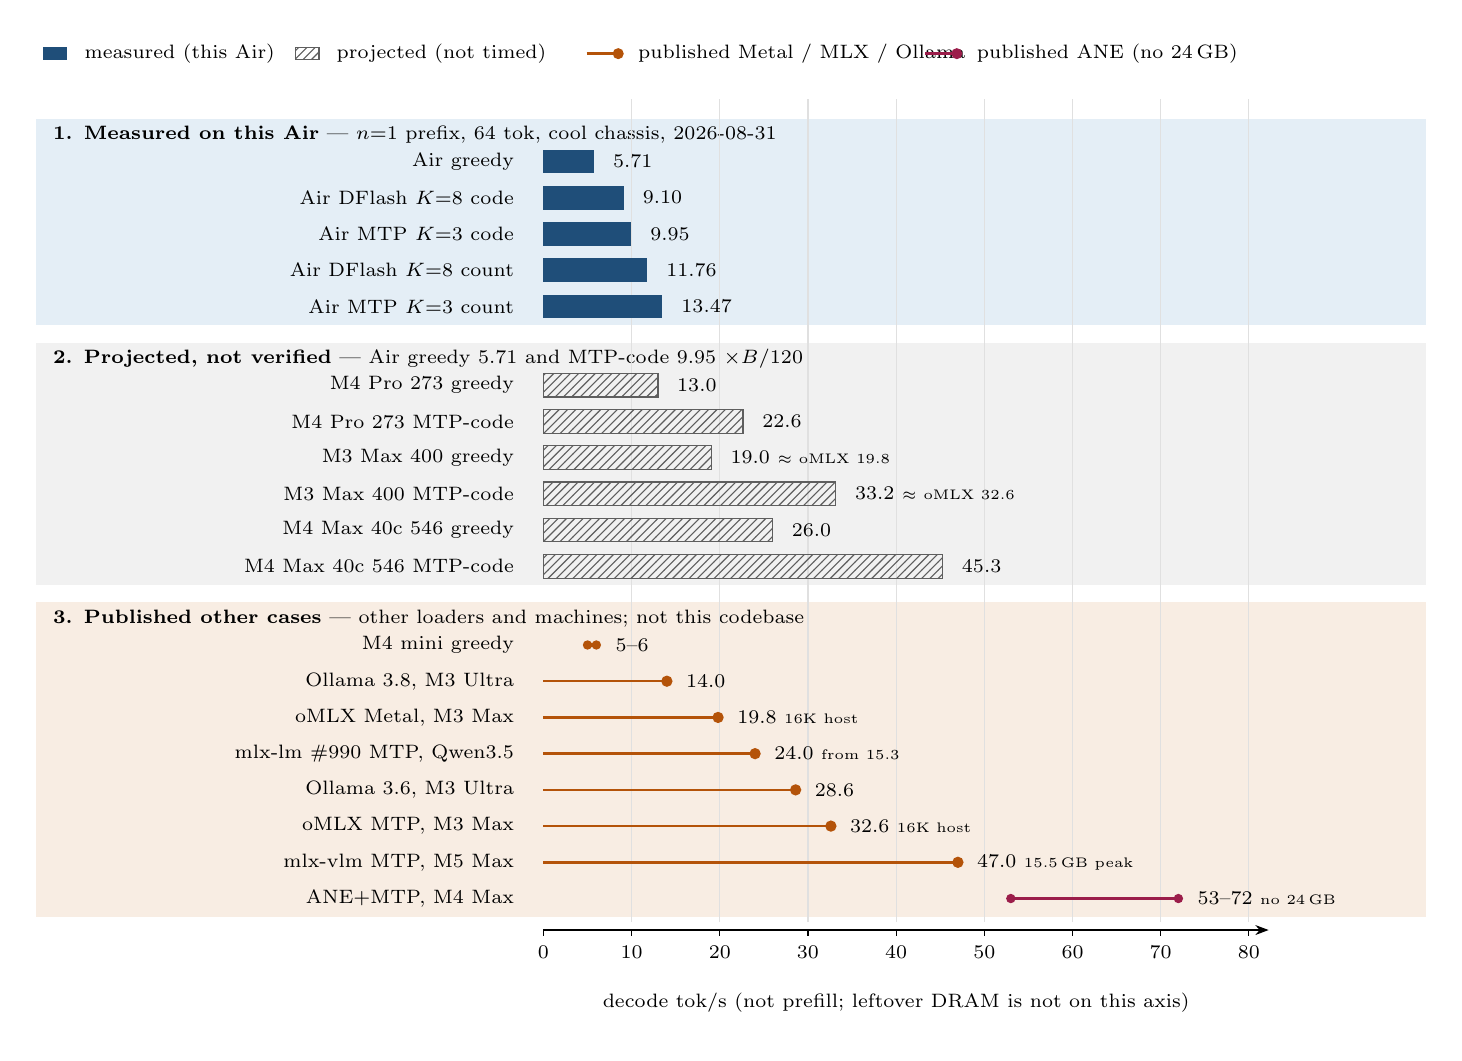
\begin{tikzpicture}[font=\scriptsize, >=Stealth]
\definecolor{meas}{HTML}{1F4E79}
\definecolor{measband}{HTML}{E4EEF6}
\definecolor{proj}{HTML}{5E5E5E}
\definecolor{projband}{HTML}{F1F1F1}
\definecolor{pub}{HTML}{B45309}
\definecolor{pubane}{HTML}{9B1D4A}
\definecolor{pubband}{HTML}{F8EDE3}
\fill[white] (-6.55,-0.85) rectangle (11.310,11.910);
\fill[pubband] (-6.45,0.610) rectangle (11.210,4.610);
\node[anchor=west, font=\scriptsize] at (-6.35,4.410) {{\textbf{3. Published other cases}} --- other loaders and machines; not this codebase};
\fill[projband] (-6.45,4.830) rectangle (11.210,7.910);
\node[anchor=west, font=\scriptsize] at (-6.35,7.710) {{\textbf{2. Projected, not verified}} --- Air greedy 5.71 and MTP-code 9.95 $\times B/120$};
\fill[measband] (-6.45,8.130) rectangle (11.210,10.750);
\node[anchor=west, font=\scriptsize] at (-6.35,10.550) {{\textbf{1. Measured on this Air}} --- $n{=}1$ prefix, 64 tok, cool chassis, 2026-08-31};
\draw[black!12] (1.120,0.55) -- (1.120,11.010);
\draw[black!12] (2.240,0.55) -- (2.240,11.010);
\draw[black!12] (3.360,0.55) -- (3.360,11.010);
\draw[black!12] (4.480,0.55) -- (4.480,11.010);
\draw[black!12] (5.600,0.55) -- (5.600,11.010);
\draw[black!12] (6.720,0.55) -- (6.720,11.010);
\draw[black!12] (7.840,0.55) -- (7.840,11.010);
\draw[black!12] (8.960,0.55) -- (8.960,11.010);
\draw[pubane, line width=1.35pt] (5.936,0.850) -- (8.064,0.850);
\fill[pubane] (5.936,0.850) circle (1.7pt);
\fill[pubane] (8.064,0.850) circle (1.7pt);
\node[anchor=east, align=right] at (-0.25,0.850) {ANE+MTP, M4 Max};
\node[anchor=west] at (8.184,0.850) {53--72 {\tiny no 24\,GB}};
\draw[pub, line width=0.9pt] (0,1.310) -- (5.264,1.310);
\fill[pub] (5.264,1.310) circle (2.05pt);
\node[anchor=east, align=right] at (-0.25,1.310) {mlx-vlm MTP, M5 Max};
\node[anchor=west] at (5.384,1.310) {47.0 {\tiny 15.5\,GB peak}};
\draw[pub, line width=0.9pt] (0,1.770) -- (3.651,1.770);
\fill[pub] (3.651,1.770) circle (2.05pt);
\node[anchor=east, align=right] at (-0.25,1.770) {oMLX MTP, M3 Max};
\node[anchor=west] at (3.771,1.770) {32.6 {\tiny 16K host}};
\draw[pub, line width=0.9pt] (0,2.230) -- (3.203,2.230);
\fill[pub] (3.203,2.230) circle (2.05pt);
\node[anchor=east, align=right] at (-0.25,2.230) {Ollama 3.6, M3 Ultra};
\node[anchor=west] at (3.323,2.230) {28.6};
\draw[pub, line width=0.9pt] (0,2.690) -- (2.688,2.690);
\fill[pub] (2.688,2.690) circle (2.05pt);
\node[anchor=east, align=right] at (-0.25,2.690) {mlx-lm \#990 MTP, Qwen3.5};
\node[anchor=west] at (2.808,2.690) {24.0 {\tiny from 15.3}};
\draw[pub, line width=0.9pt] (0,3.150) -- (2.218,3.150);
\fill[pub] (2.218,3.150) circle (2.05pt);
\node[anchor=east, align=right] at (-0.25,3.150) {oMLX Metal, M3 Max};
\node[anchor=west] at (2.338,3.150) {19.8 {\tiny 16K host}};
\draw[pub, line width=0.9pt] (0,3.610) -- (1.568,3.610);
\fill[pub] (1.568,3.610) circle (2.05pt);
\node[anchor=east, align=right] at (-0.25,3.610) {Ollama 3.8, M3 Ultra};
\node[anchor=west] at (1.688,3.610) {14.0};
\draw[pub, line width=1.35pt] (0.560,4.070) -- (0.672,4.070);
\fill[pub] (0.560,4.070) circle (1.7pt);
\fill[pub] (0.672,4.070) circle (1.7pt);
\node[anchor=east, align=right] at (-0.25,4.070) {M4 mini greedy};
\node[anchor=west] at (0.792,4.070) {5--6};
\fill[pattern=north east lines, pattern color=proj] (0,4.920) rectangle (5.071,5.220);
\draw[proj, thin] (0,4.920) rectangle (5.071,5.220);
\node[anchor=east, align=right] at (-0.25,5.070) {M4 Max 40c 546 MTP-code};
\node[anchor=west] at (5.191,5.070) {45.3};
\fill[pattern=north east lines, pattern color=proj] (0,5.380) rectangle (2.910,5.680);
\draw[proj, thin] (0,5.380) rectangle (2.910,5.680);
\node[anchor=east, align=right] at (-0.25,5.530) {M4 Max 40c 546 greedy};
\node[anchor=west] at (3.030,5.530) {26.0};
\fill[pattern=north east lines, pattern color=proj] (0,5.840) rectangle (3.715,6.140);
\draw[proj, thin] (0,5.840) rectangle (3.715,6.140);
\node[anchor=east, align=right] at (-0.25,5.990) {M3 Max 400 MTP-code};
\node[anchor=west] at (3.835,5.990) {33.2 {\tiny $\approx$ oMLX 32.6}};
\fill[pattern=north east lines, pattern color=proj] (0,6.300) rectangle (2.132,6.600);
\draw[proj, thin] (0,6.300) rectangle (2.132,6.600);
\node[anchor=east, align=right] at (-0.25,6.450) {M3 Max 400 greedy};
\node[anchor=west] at (2.252,6.450) {19.0 {\tiny $\approx$ oMLX 19.8}};
\fill[pattern=north east lines, pattern color=proj] (0,6.760) rectangle (2.535,7.060);
\draw[proj, thin] (0,6.760) rectangle (2.535,7.060);
\node[anchor=east, align=right] at (-0.25,6.910) {M4 Pro 273 MTP-code};
\node[anchor=west] at (2.655,6.910) {22.6};
\fill[pattern=north east lines, pattern color=proj] (0,7.220) rectangle (1.455,7.520);
\draw[proj, thin] (0,7.220) rectangle (1.455,7.520);
\node[anchor=east, align=right] at (-0.25,7.370) {M4 Pro 273 greedy};
\node[anchor=west] at (1.575,7.370) {13.0};
\fill[meas] (0,8.220) rectangle (1.509,8.520);
\node[anchor=east, align=right] at (-0.25,8.370) {Air MTP $K{=}3$ count};
\node[anchor=west] at (1.629,8.370) {13.47};
\fill[meas] (0,8.680) rectangle (1.317,8.980);
\node[anchor=east, align=right] at (-0.25,8.830) {Air DFlash $K{=}8$ count};
\node[anchor=west] at (1.437,8.830) {11.76};
\fill[meas] (0,9.140) rectangle (1.114,9.440);
\node[anchor=east, align=right] at (-0.25,9.290) {Air MTP $K{=}3$ code};
\node[anchor=west] at (1.234,9.290) {9.95};
\fill[meas] (0,9.600) rectangle (1.019,9.900);
\node[anchor=east, align=right] at (-0.25,9.750) {Air DFlash $K{=}8$ code};
\node[anchor=west] at (1.139,9.750) {9.10};
\fill[meas] (0,10.060) rectangle (0.640,10.360);
\node[anchor=east, align=right] at (-0.25,10.210) {Air greedy};
\node[anchor=west] at (0.760,10.210) {5.71};
\draw[->] (0,0.45) -- (9.210,0.45);
\draw (0.000,0.45) -- ++(0,-0.08) node[below, font=\scriptsize] {0};
\draw (1.120,0.45) -- ++(0,-0.08) node[below, font=\scriptsize] {10};
\draw (2.240,0.45) -- ++(0,-0.08) node[below, font=\scriptsize] {20};
\draw (3.360,0.45) -- ++(0,-0.08) node[below, font=\scriptsize] {30};
\draw (4.480,0.45) -- ++(0,-0.08) node[below, font=\scriptsize] {40};
\draw (5.600,0.45) -- ++(0,-0.08) node[below, font=\scriptsize] {50};
\draw (6.720,0.45) -- ++(0,-0.08) node[below, font=\scriptsize] {60};
\draw (7.840,0.45) -- ++(0,-0.08) node[below, font=\scriptsize] {70};
\draw (8.960,0.45) -- ++(0,-0.08) node[below, font=\scriptsize] {80};
\node[anchor=north] at (4.480,-0.22) {decode tok/s (not prefill; leftover DRAM is not on this axis)};
\fill[meas] (-6.35,11.500) rectangle (-6.05,11.660);
\node[anchor=west] at (-5.95,11.580) {measured (this Air)};
\fill[pattern=north east lines, pattern color=proj] (-3.15,11.500) rectangle (-2.85,11.660);
\draw[proj] (-3.15,11.500) rectangle (-2.85,11.660);
\node[anchor=west] at (-2.75,11.580) {projected (not timed)};
\draw[pub, line width=0.9pt] (0.55,11.580) -- (0.95,11.580);
\fill[pub] (0.95,11.580) circle (2pt);
\node[anchor=west] at (1.08,11.580) {published Metal / MLX / Ollama};
\draw[pubane, line width=1.2pt] (4.85,11.580) -- (5.25,11.580);
\fill[pubane] (5.25,11.580) circle (2pt);
\node[anchor=west] at (5.38,11.580) {published ANE (no 24\,GB)};
\end{tikzpicture}

}
\caption{Dense 27B-class decode, three categories. (1)~Measured on this M4 Air, one prefix. (2)~Unverified $B/120$ cartoons. (3)~Published other loaders. The 13.47 count pin is not scaled. RAM${-}15.1$\,GiB is omitted.}
\label{fig:bw}
\end{figure}

\begin{table}[t]
\centering
\caption{Tiers corresponding to Figure~\ref{fig:bw}. Extra RAM does not make the 15\,GiB pack larger; it changes room for OS, prefill, vision, and alternative compiled paths. Projected tok/s follow bandwidth.}
\label{tab:proj}
\small
\begin{tabular}{@{}lrrrrr@{}}
\toprule
Tier & UM (GB) & BW (GB/s) & Greedy & MTP-code & Status \\
\midrule
M4 Air & 24 & 120 & 5.71 & 9.95 & measured \\
M4 Pro & 48 & 273 & 13.0 & 22.6 & projected \\
M3 Max & 128 & 400 & 19.0 & 33.2 & projected ${\approx}$ oMLX 19.8 / 32.6 \\
M4 Max (40c) & 128 & 546 & 26.0 & 45.3 & projected \\
\bottomrule
\end{tabular}
\end{table}

\begin{table}[t]
\centering
\caption{oMLX M3 Max 128\,GB~\citep{omlx2874} scaled by $120/400$ versus this Air. Prefill does not sit on the same line as decode: ANE 267 would scale to a fictional 80; this Air measures ${\approx}48$ without ANE.}
\label{tab:scale}
\small
\begin{tabular}{@{}lrrr@{}}
\toprule
Quantity & M3 Max & ${\times}0.30$ & Air measured \\
\midrule
Metal decode & 19.8 & 5.94 & 5.71 \\
MTP decode & 32.6 & 9.78 & 9.95 (code) \\
Metal prefill & 115 & 34.5 & 48 \\
ANE prefill & 267 & 80 & 48 (no ANE) \\
\bottomrule
\end{tabular}
\end{table}

\FloatBarrier

%======================================================================
\section{Discussion and Limitations}
\label{sec:discuss}

Most mechanisms here are not new in isolation. MTP is Qwen’s~\citep{qwen3}; lossless speculation is Leviathan--Chen~\citep{leviathan2023speculative,chen2023accelerating}; fused Metal GDN is MLX~\citep{mlx2023,mlxlm}; prefix caching is established~\citep{zheng2024sglang}; expert caching predates this runtime~\citep{rajbhandari2022deepspeed,he2022fastermoe}. The result is how they interact on a machine small enough that the usual abstractions break.

The sparse path shows that unified memory is not discrete VRAM with a larger address. A larger expert cache can cut miss rate and still cut throughput. The dense path shows the other side: once 4-bit fits, another streaming layer is waste. Hybrid state adds a correctness boundary. That is the novelty claim. \slotbank{} does not claim a new kernel, quantizer, or routing method.

Table~\ref{tab:reject} lists attractive speedups that are out of scope here: extra residency, a different model, or a changed prompt.

\begin{table}[t]
\centering
\caption{Acceleration paths excluded by the target model or the 24\,GB envelope.}
\label{tab:reject}
\scriptsize
\begin{tabular}{@{}p{3.4cm}p{4.2cm}p{5.6cm}@{}}
\toprule
Lever & Published / expected & Why not here \\
\midrule
oMLX ANE prefill & $83{\to}274$ tok/s~\citep{weschera2026} & Second compiled residency; 64--128\,GB \\
Ollama MLX 0.19 & ${+}93\%$ decode~\citep{ollama019} & 35B-A3B NVFP4, M5, 32\,GB+ \\
CUDA chunked GDN & $8.5{\times}$ TTFT~\citep{mlxvlm1423} & Metal already fused; not an Air win \\
SpecPrefill / SwiftKV & $2$--$7{\times}$ TTFT~\citep{yuan2024specprefill,swiftkv} & Drops prompt or trained compute \\
4B as 27B drafter & cheaper draft & Different width/vocab; unsafe rewind \\
Forced $K{=}5$ on 27B & larger block & Not the trained $K$ of either 27B drafter \\
Hybrid KV paging & longer apparent context & GDN cannot be trimmed equivalently \\
\bottomrule
\end{tabular}
\end{table}

Every uncited 27B and 35B number is one fanless Air. Bandwidth scaling that matches decode here is not a law for the next M-series chip. Cool-machine tables overstate soak: after 8--10 minutes this chassis sits at roughly 60--70\% of those peaks; that observation was not retimed as a formal curve. First pin is about 30\,s. ``Fits'' means admission plus a generate that does not jetsam, not unlimited multitasking. 4-bit is not bf16. Vendor cards (SWE-bench, GPQA) describe the vendor harness, not this machine.

%======================================================================
\section{Related Work}
\label{sec:related}

Related work is necessary because the claim is an intersection, not a new primitive. The systems below are the ones this design is \emph{not}.

vLLM, SGLang, DistServe, Splitwise, and QServe assume a discrete GPU heap and, usually, pageable attention state~\citep{kwon2023vllm,zheng2024sglang,zhong2024distserve,patel2024splitwise,lin2024qserve}. DeepSpeed-MoE, FasterMoE, and expert parallelism treat experts as a sharded, prefetchable resource across devices~\citep{rajbhandari2022deepspeed,he2022fastermoe}. Those designs have a copy engine and a heap that is not also the file cache. \slotbank{} sizes a resident window so the rest of the bank can remain evictable pages on one worker. GPTQ, AWQ, and SmoothQuant are consumed as community affine-4 packs~\citep{frantar2023gptq,lin2024awq,xiao2024smoothquant}; this paper does not requantize.

Leviathan--Chen, Medusa, EAGLE, and Qwen MTP are the speculation lineage~\citep{leviathan2023speculative,chen2023accelerating,cai2024medusa,li2024eagle,qwen3}. llama.cpp \texttt{draft-mtp} and mlx-lm PR~990 connect the head~\citep{ctaylor83mtp,mlxlm990}. The systems problem on hybrid GDN is rewind, not the existence of a head. vLLM’s \texttt{mamba\_cache\_mode=all} checkpoints SSM state so a mid-prompt hit can restore~\citep{vllm36649}; the Metal GDN kernel does not return those intermediates. SpecPrefill, SwiftKV, and PyramidKV change the prompt or compress KV~\citep{yuan2024specprefill,swiftkv,pyramidkv}. The keep-set shape is reused here only as an admission policy for which token ids are prefills, and only in the long-prompt case study.

\texttt{mlx-lm}, \texttt{mlx-vlm}, llama.cpp, Ollama, and oMLX are the native Mac stacks~\citep{mlx2023,mlxlm,mlxvlm,llamacpp,ollama019,omlx2874}. Community benches mix clocks and machines~\citep{terminalbytes2026,orcarouter2026,weschera2026,nathanmaine}. mlx-vlm PR~1423’s $8.5{\times}$ TTFT is CUDA chunked GDN; Metal already fuses the time loop when $D_k \bmod 32 = 0$~\citep{mlxvlm1423}.

%======================================================================
\section{Conclusion}
\label{sec:conc}

Unified memory is not a discrete GPU with a nicer name, and hybrid GDN is not a KV cache with a smaller footprint. Those two facts, not a missing flag, are why a 15\,GiB 27B and a 19\,GiB 35B-A3B are still systems problems after the checkpoint has downloaded.

\slotbank{} answers them with two residency paths and one correctness contract. MoE banks that do not fit are served through a slot pack whose capacity $C$ is chosen so the OS page cache remains useful; $C{=}32$ is the measured interior maximum on this Air. Dense 27B does not install slots. Speculative decode uses a rollback that can restore hybrid state. Prefix reuse restores only exact stored snapshots, which is why an 819-token follow-up is 0.88\,s when the prefix matches and 17.0\,s when it does not.

On this Air that is enough to run a 35B-A3B that stock MLX thrashes and llama.cpp at matching Q4 does not run (4.2 cold / 6.1 warm at ${\approx}3.8$\,GiB wired), and enough to put dense 27B greedy decode on the $120/400$ scaling of published Max Metal numbers (5.71 measured vs.\ 5.94 predicted). Doubling the slot pack to 64 cuts misses and still reads more disk. That is the result I would keep if the rest of the manuscript were deleted.

The study is one fanless machine. A 48-prompt Metal sweep, a five-repeat capacity experiment, a controlled thermal curve, and a second unified-memory capacity are what a broader evaluation still owes.

\section*{Acknowledgements}

The author thanks the mlx-lm, mlx-vlm, oMLX, Ollama, and Qwen contributors for kernels, checkpoints, and published measurements. Errors in interpretation, and all uncited M4 Air measurements, are the author’s.

\bibliographystyle{plainnat}
\bibliography{refs}

\appendix
\section{Notation}
\label{app:notation}

\begin{center}
\small
\begin{tabular}{@{}ll@{}}
\toprule
Symbol & Meaning \\
\midrule
$C$ & Resident expert slots (MoE path only) \\
$K$ & Trained speculative block length (MTP $3$, DFlash2 $8$, 4B DFlash $5$) \\
$B$ & Delivered bandwidth of the active tier \\
$W_{\mathrm{touch}}$ & Bytes read per token \\
$S_t$ & Gated DeltaNet matrix state after token $t$ \\
$p$ & Exact stored prefix (token ids) \\
$\alpha_i$ & Leviathan--Chen acceptance of draft token $i$ \\
bpw & Average stored bits per weight after quantization \\
\bottomrule
\end{tabular}
\end{center}

\section{Software campaign}
\label{app:campaign}

Campaign \texttt{20260902T001357Z} is a host-side drift check: import fence, catalog, and recorded pins. It ran on Linux x86\_64 with no Metal 27B weights (29/29 paper-claim tests; 221 filtered CI tests passed). It is included so a reader can see that the software contract was checked on the compilation host. It is not a hardware evaluation and is not required to read the results in \S\ref{sec:eval}.

\section{Sparse-path token budget}
\label{app:budget}

After \texttt{preadv} and \texttt{memoryview}, the remaining per-token budget on Qwen3.5-35B-A3B is still I/O-shaped. The structural limit is that layer $L$'s expert set is unknown until layer $L{-}1$ completes.

\begin{center}
\small
\begin{tabular}{@{}lrl@{}}
\toprule
Term & ms/token & Source \\
\midrule
GPU compute & ${\sim}50$ & Metal; consistent with 19--21 tok/s stubbed ceiling \\
Device I/O, depth 8 & ${\sim}46$--48 & kernel + SSD \\
Host memcpy + Metal allocation & ${\sim}14$ & libc / MLX allocator \\
Command-buffer stall & ${\sim}15$--25 & driver \\
Redundant \texttt{.item()} (fixed) & ${\sim}7$--11 & extra Metal synchronization \\
Thread pool & ${\sim}7$ & Python scheduling \\
MLX graph construction & ${\sim}5$--8 & MLX C++ \\
CPython bytecode & ${\sim}3$--5 & interpreter \\
\bottomrule
\end{tabular}
\end{center}

\section{Reporting checklist}
\label{app:checklist}

A citation of a local-serving number should record: chip and unified memory; advertised Metal working set and bandwidth; checkpoint id and quantization; draft sidecar and trained $K$ if any; loader and rollback primitive; leave-free reserve; clock name (cold e2e, warm decode, TTFT, follow-up TTFT, or compute-only); cache hit or miss; thermal state; and the correctness oracle. Temperature 1.0 from a client is not a greedy benchmark.

\end{document}
